\documentclass[10pt]{exam}
\usepackage[hon]{template-for-exam}
\usepackage{enumitem,multicol,multirow,tikz,fancybox,graphicx}
\usetikzlibrary{shadings,decorations.pathmorphing,arrows.meta,patterns,calc}
\setlist[enumerate,itemize]{topsep=0pt,itemsep=-1ex,partopsep=1ex,parsep=1ex}
\graphicspath{{./figures}}

\title{Measuring $g$ Using a Bouncing Tennis Ball}
\author{Rohrbach}
\date{\today}

\begin{document}
\maketitle

\section*{Purpose}

Use the graphs of motion for a ball that is in free fall to measure the acceleration of gravity $g$.


\section*{Procedure}

\begin{enumerate}
  \item Plug the LabQuest Mini into your computer
  \item Download \texttt{Measuring-g-lab.gambl} from Schoology and open it in \texttt{Graphical Analysis}.
  \item Hold the ball about 50 cm away from the motion detector.  Start taking data, and then drop the ball, allowing it to bounce a few times.
  \item See if your data looks smooth.  If there have been issues, take a new data set before proceeding.
\end{enumerate}

\section*{Data}

Sketch the position and velocity graphs below.  Please \textbf{be careful} with the horizontal axis.  Try to make it so that each graph has the same events occuring at the same location along the $t$-axis.  Don't rush this step.

\hfill 

    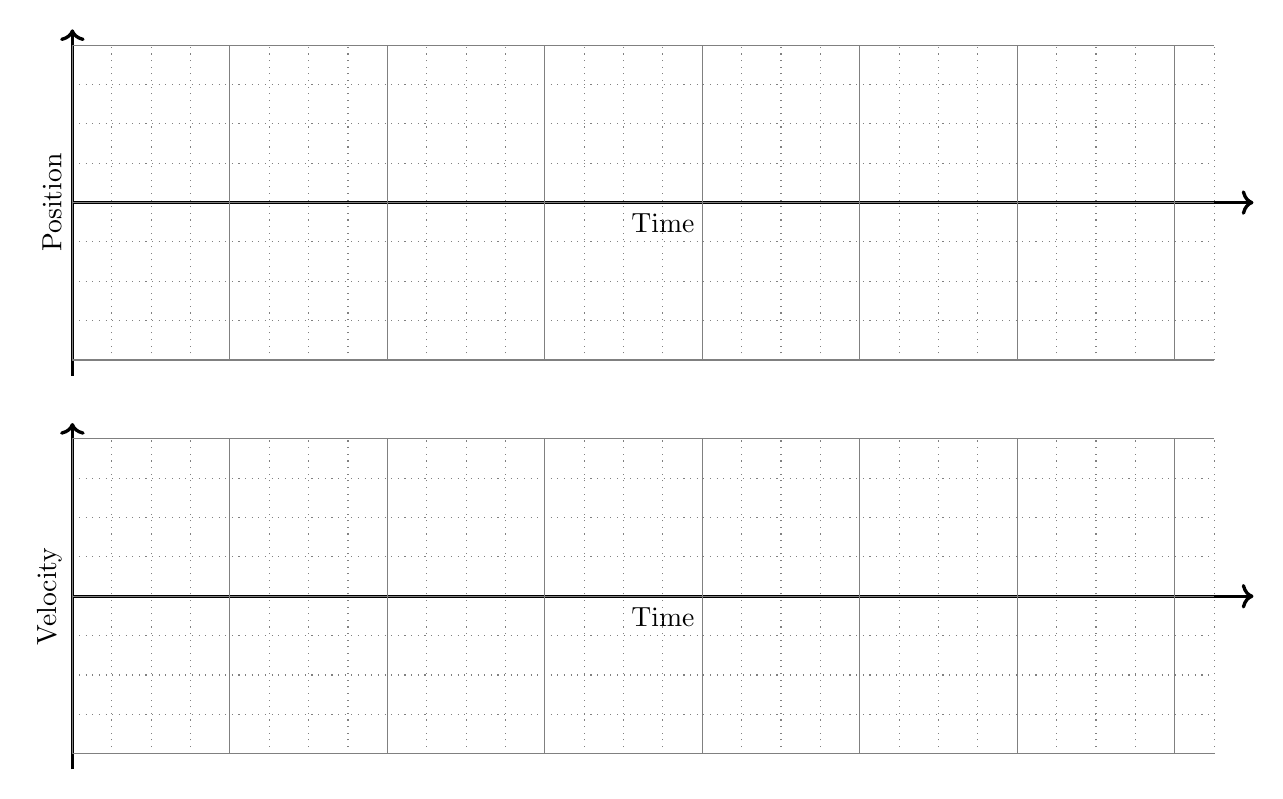
\begin{tikzpicture}
      \newcommand{\drawgraph}[2]{
        \draw[->,very thick] (0,#2) +(0,-2.2) -- +(0,2.2)
          node[midway, above, sloped, fill=white] 
          {#1};
        \draw[->,very thick] (0,#2) -- +(15,0) 
          node[midway, below] {Time};
        \draw[gray,thin,dotted,shift={(0,#2)}] 
          (0,-2) grid[step=0.5] ++(14.5,4);
        \draw[gray,shift={(0,#2)}] 
          (0,-2) grid[step=2] ++(14.5,4);
      }

      \drawgraph{Position}{0}
      \drawgraph{Velocity}{-5}



    \end{tikzpicture}


\pagebreak

\section*{Analysis}

\begin{enumerate}[resume]
  \item On each graph, label all ``interesting'' times.  For example, label when the original drop time is, when the bounces occur, and when the maximum heights occur.
  \item Explain why each graph makes sense given the motion of the ball.
  \begin{itemize}
    \item Postion graph \vs 
    \item Velocity graph \vs
    \item Acceleration graph \vs
  \end{itemize}

  \item What does a linear segment of a velocity vs. time graph indicate? What is the significance of the slope of that linear segment? \vs 
  \item The velocity graph should be linear in the region where the ball was in freefall. Fit a linear equation to your data in this region.
  
  \begin{itemize}
    \item Select the data in the region that corresponds to when the ball was in freefall.
    \item Click Graph Tools, 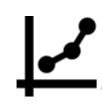
\includegraphics[height=1.2em]{graph-tools}, for the velocity graph and choose Apply Curve Fit.
    \item Select Linear as the curve fit and click Apply. 
  \end{itemize}

  Write down the equation for the best fit line:  \vs
  
  \item Use your best fit equation to identify the measured value of $g$. \vs 
  \item Calculate percent error based on the expected value for $g$.
  %
  \begin{align*}
    \text{Percent Error} = \frac{\left| \text{measured} - \text{expected}  \right|}{\text{expected}} \times 100\%
  \end{align*}
  %
  \vs

\end{enumerate}



\pagebreak

\section*{Conclusion}

Write a paragraph explaining your results on the lab.  Your paragraph should address: (1) Explain what experiment you diad and what graphs you made; (2) Explain what the graphs look like and why those shapes made sense; (3) Explain how you got your measured value for $g$ and a report of the percent error compared to the expected value; and (4) Identify three to four factors that could have created uncertainties in your measurements and explain how each factor may have influenced your percent error.



\end{document}